\section{Durchführung}
\label{sec:Durchführung}

Der verwendete Versuchsaufbau ist in Abbildung ? zu sehen.\\
\begin{figure}[h]
    \centering
    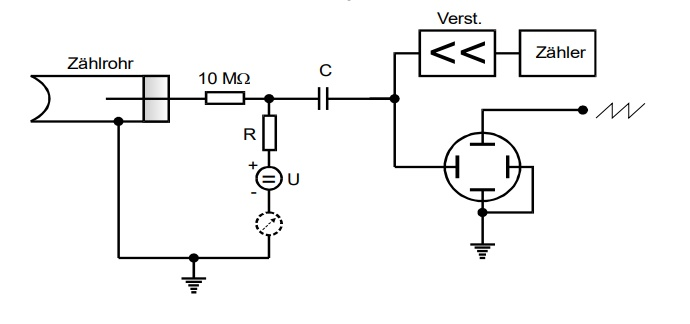
\includegraphics{Aufbau.jpg}
    \caption{Skizze der Messapparatur}
    \label{fig:Skizze der Messapparatur}
\end{figure}\\
Vor dem Zählrohr wird eine r ^{204}Tl-Quelle aufgebaut, so dass die Zählrate bei einer mittleren Zählrohrspannung nicht größer als 100 Imp/s ist.
Die Beschränkung der Zählrate ist nötig, um Totzeit-Korrekturen zu vermeiden.\\
Nun wird nach jeder Messung der Anzahl der Zerfälle die am Zählrohr anliegende Spannung um 10 V erhöht.\\
Parallel zu dieser Messung wird außerdem mit einem Abstand von 50 V der Zählrohrstrom I notiert.\\
Anschließend soll die Totzeit bestimmt werden. Dies wird zuerst mit der Zwei-Quellen-Methode realisiert. Dazu muss die Quelle mit einem geringeren Abstand zum Zählrohr plaziert werden. Nacheinander werden die Quelle $Q_1$, die Quellen $Q_1$ und $Q_"$ gemeinsam und nur die Quelle $Q_2$ vor dem Zählrohr aufgebaut
und die zugehörigen Zählraten aufgenommen.\\
Danach wird die Bestimmung der Totzeit mit Hilfe eines Oszilloskops durchgeführt. Dazu wird die von den Zählrohrimpulsen abhängige Zeitablenkung des Oszillographens genutzt.\\
